\section{Einleitung}
Der Einsatz von Robotern prägt zunehmend den Arbeitsmarkt und beeinflusst die Art und Weise wie Unternehmen ihre Prozesse gestalten. Diese Entwicklung beschränkt sich nicht nur auf klassische Einsatzgebiete wie die Industrie, in der beispielsweise Montageroboter eingesetzt werden, und den Verbrauchermarkt, in dem Staubsaugerroboter weit verbreitet sind, sondern zunehmened auch auf die Dienstleistungsbranche. So ist der Absatz an Service Robotern für professionelle Anwendungen 2022 laut der \ac{IFR} um 48\% gestiegen \cite{IFR2023}. In der Industrie ist der Absatz 2022 im Vergleich schwächer gestiegen \cite[S.~9]{WorldRobotics2023} und im Verbrauchermarkt sogar gesunken \cite[S.~37]{WorldRobotics2023}. Das Wachstum des Absatzes wird laut der \ac{IFR} durch eine gesteigerte Nachfrage getrieben, die unter anderem auf einen Mangel an Arbeitskräften zurückzuführen ist \cite[S.~36]{WorldRobotics2023}. Laut der \ac{BA} ist die Menge unbesetzter Arbeitsplätze in Deutschland in den letzten 10 Jahren um ~40\% gestiegen und - trotz des Rückgangs um ~18\% in den letzten zwei Jahren - weiter auf einem hohen Stand \cite{BA2024}. Insbesondere in der Gastronomie gibt es einen erheblichen Personalmangel, der zum Teil auf die Corona-Pandemie zurückzuführen ist, da in dieser Zeit viele Angestellte in andere Berufsfelder gewechselt sind. Laut dem Institut der deutschen Wirtschaft, welches sich auf Daten der \ac{BA} bezieht, sind während des Pandemiejahrs 2020 ~216.000 Arbeiter aus dem Gastgewerbe in ein anderes Berufsfeld gewechselt \cite{BA2024}. Service Roboter bieten durch eine effiziente Unterstützung des Personals die Möglichkeit den Personalmangel zu mitigieren. So ersetzen Service Roboter das Personal meistens nicht vollständig, sondern unterstützen es, sodass es mehr Zeit für andere Aufgaben wie die Kundenbetreuung hat \cite[S.~271-272]{Sprenger2015}. In der Gastronomie können Lieferroboter beispielsweise bestimmte Kellneraufgaben übernehmen und so das Personal entlasten.

\subsection{Hintergrund und Motivation}
In diesem Kontext hat sich die Firma Tobit Laboratories AG entschieden die Potenziale von Lieferrobotern für eigene Gastronomiestandorten zu erkunden. So hat das Unternehmen mehrere Lieferroboter von Pudu Robotics erworben, um diese Technologie zu testen. Zur Steuerung der Roboter aber auch zur Erweiterung der Funktionen wurde das \ac{BCB} entwickelt, das im Kapitel \ref{sec:BotControlBackend} näher erläutert wird. Die Roboter sollen zunächst im Firmengebäude für kleinere Botengänge eingesetzt werden und potenziell später an verschiedenen Gastronomiestandorten eingesetzt werden. Hierfür muss zum einen die Navigationsfähigkeit und Zuverlässligkeit geprüft werden, gleichzeitig muss aber auch eine intuitive Anwendung entstehen, mit der die Roboter gesteuert und verwaltet werden können.

\subsection{Zielsetzung und Forschungsfrage}
Diese Arbeit setzt an diesem Punkt an und zielt darauf ab, eine Anwendung zu konzipieren und prototypisch zu implementieren, die die Steuerung und Verwaltung von Lieferrobotern ermöglicht und zudem eine Übersicht über deren Positionen bietet. Bei der Anwendung soll es sich um eine Webanwendung handeln, die im Gegensatz zu nativen Anwendungen eine plattformunabhängige Nutzung und sofortigen Verfügbarkeit ohne Download und Installation bietet. Für eine möglichst übersichtliche Darstellung der Roboterpositionen sollen 3D-Modelle der Gebäude - in denen sich die Roboter befinden - genutzt werden. Da die Roboter potenziell in verschiedenen Gastronomiestandorten eingesetzt werden sollen, sollte das Erzeugen der 3D-Modelle mit möglichst wenig Aufwand verbunden sein. Trotz des erhöhten Rechenaufwands, der mit der Darstellung von 3D-Modelle verbunden ist, soll die Anwendung möglichst performant sein.
% TODO Webanwendung Quelle

Die Forschungsfrage lautet demnach: Wie kann eine effiziente und benutzerfreundliche Steuerung und Verwaltung von Servicerobotern implementiert werden? Ein zusätzlicher Schwerpunkt liegt auf der Methode zur einfachen Generierung von 3D-Gebäude- oder Raummodellen, da diese die Grundlage für die nutzerfreundliche Visualisierung in der Webanwendung schaffen soll. Es ist anzumerken, dass die genutzte Methode nicht zwingend in die Webanwendung integriert werden muss.

\subsection{Methodik}
Der Einsatz wissenschaftlicher Methoden orientiert sich in dieser Arbeit an dem \ac{DSR} Ansatz nach Hevner \cite{Hevner2004}. Der Ansatz bietet einen Rahmen für \ac{DSR} im Bereich der Informationssysteme und ist somit für diese Arbeit geeignet. Grundsätzlich ist \ac{DSR} ein iterativer Forschungsansatz, mit dem Lösungen für praktische Probleme, mithilfe der Entwicklung von Artefakten gefunden werden. In dem Rahmen dieser Arbeit ist das Artefakt der zu entwickelnde Prototyp.

\subsubsection{Design Science Research nach Hevner}
Bei diesem Abschnitt handelt es sich um eine Zusammenfassung des \ac{DSR} Ansatzes nach Hevner \cite[S.~79-81]{Hevner2004}. Hevners Ansatz setzt sich aus drei Zyklen zusammen:

\begin{itemize}
    \item Relevanz-Schleife
    \item Strenge-Schleife
    \item Design-Schleife
\end{itemize}

Die Relevanz- und Strengeschleifen erfüllen eine unterstützende Funktion, um sicherzustellen, dass die Entwicklung des Artefakts verschiedenen Anforderungen gerecht wird. Aus der Relevanz Schleife ergeben sich - basierend auf der Umgebung, für die das Artefakt entwickelt wird - die Anforderungen an den Inhalt und die Qualität des Artefakts. Währenddessen ergeben sich aus der Strenge-Schleife die Anforderungen an die wissenschaftlichen Methoden und Standards, die während der Entwicklung eingesetzt werden und mit denen das Artefakt evaluiert wird. In der Design-Schleife wechseln sich währenddessen die Entwicklung und Auswertung des Artefakts iterativ ab. In der Abbildung ref{fig:DesignScienceResearch} wird dieser Prozess grafisch dargestellt, wodurch die Funktion und Stellung der Elemente verdeutlicht wird. So sieht man das die Relevanz- und Design-Schleifen als Unterstützungsprozesse für den Designprozess dienen.

\begin{figure}[H]
    \caption{Design Science Research nach Hevner}\label{fig:DesignScienceResearch}
    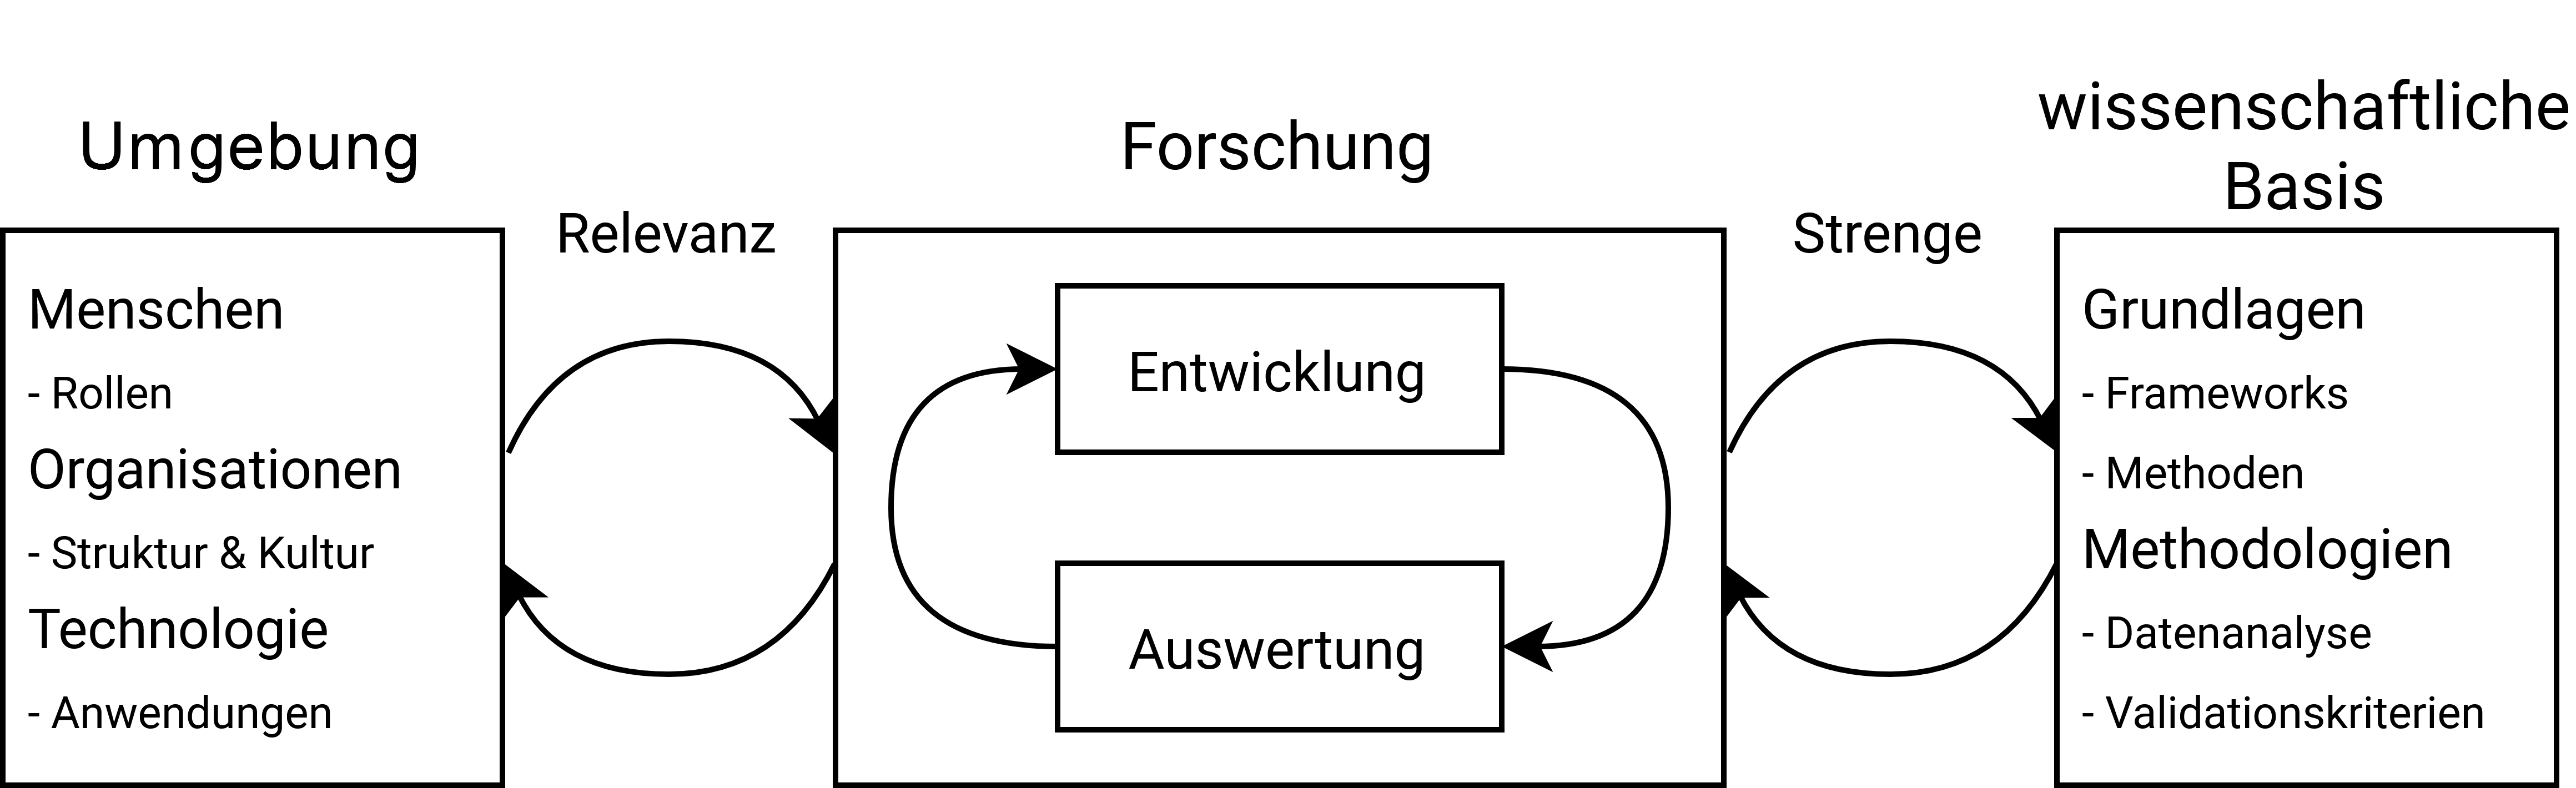
\includegraphics[width=0.9\textwidth]{Design Science Research.png}
    \\
    % TODO Check if "et al." is right
    Quelle: In Anlehnung an Hevner et al. \cite[S.~80]{Hevner2004}
\end{figure}

\subsubsection{Design Science Research im Rahmen der Arbeit}

Die Prozesse des \ac{DSR} Ansatz nach Hevner werden in dieser Arbeit durch verschiedene wissenschaftliche Methoden abgebildet.

\paragraph{Literaturrecherche}
Im ersten Schritt wird eine systematische Literaturrecherche durchgeführt mit der das grundlegende Verständnis über die Umgebung und die Basis an wissenschaftlichen Methoden geschaffen werden soll. So wird zum einen Wissen zu Service Robotern aber zusätzlich auch Wissen zu der Generierung von 3D-Modellen gesammelt. Auch wird Wissen zur wissenschaftlichen Auswertung von Software-Anwendungen gesammelt. Während der Implementierung des Prototyps weitet sich diese Literaturrecherche weiter auf Themengebiete aus, welche zur Lösung von Problemen relevant sind, die während der Implementierung auftreten.

\paragraph{Anforderungsanalyse}
Die Umgebungsanforderungen werden nach der Wissensfindung über eine kurze Anforderungsanalyse definiert. Diese kann auf die funktionalen und nicht funktionalen Anforderungen aufgebaut werden, die sich bereits aus der Zielsetzung und der Formulierung der Forschungsfrage ergeben. So stehen die Anforderungen, dass der Prototyp eine Webanwendung sein und eine dreidimensionale Visualisierung bieten soll bereits fest. Auch steht bereits fest, dass der Prototyp benutzerfreundlich und effizient sein soll.

\paragraph{Umsetzung}
Die Implementierung des Prototyps soll im Verfahren des Rapid Prototypings durchgeführt werden. So wechseln sich die Entwicklung und Auswertung der benutzerfreundlickeit und effizienz iterativ ab bis ein Prototyp entstanden ist, der die definierten Anforderungen erfüllt.
% TODO Quelle Rapid Prototyping
